\documentclass[a4paper,12pt]{article}

\input{lab_Preamble.tex}


\begin{document}
\author{Рябых Владислав и Исыпов Илья, Б05-905}
\title{\tbf{3.4.1.(4.13) Измерение магнитной восприимчивости диа- и парамагнетиков}}
\maketitle

\tbf{Цель работы:} измерение магнитной восприимчивости диа- и парамагнитного образцов.

\tbf{В работе используются:} электромагнит, аналитические весы, милливеберметр, источник питания постоянного тока, образцы диа- и парамагнетиков.


\section*{Теория}
копипаст из лабника/готового теха
используем формулу
\begin{equation}
	\text{что-то} = \dfrac{x}{y}
	\label{eq1}
\end{equation}

\section*{Экспериментальная установка}
(если она указана отдельно в лабнике/описании) также копипаст

\section*{Ход работы}
Делаем что-то по каким-то идеям. Рассчитываем что-то по формуле $\text{что-то} = \dfrac{x}{y}$, расчитываем погрешность как $\sigma_\text{что-то} = \text{что-то} \cdot \sqrt{\sigma_x^2 + \sigma_y^2}$. Результаты измерений приведены в таблице \ref{tab1}.

\begin{center}
\begin{tabular}{|c|c|c|c|c|c|c|c|c|c|}
	\hline
	$x$, A & 0.25 & 0.60 & 0.95 & 1.30 & 1.65 & 2.00 & 2.35 & 2.70 & 3.05 \\
	\hline
	$\Delta x$, А & 0.02 & 0.02 & 0.02 & 0.03 & 0.03 & 0.03 & 0.03 & 0.03 & 0.04 \\
	\hline
	$y$, мВб & 0.60 & 1.40 & 2.30 & 3.10 & 3.90 & 4.70 & 5.40 & 6.10 & 6.60 \\
	\hline
	$\Delta y$, мВб & 0.60 & 1.40 & 2.30 & 3.10 & 3.90 & 4.70 & 5.40 & 6.10 & 6.60 \\
	\hline
	$\text{что-то}$, Tл & 0.08 & 0.19 & 0.32 & 0.43 & 0.54 & 0.65 & 0.75 & 0.85 & 0.92 \\
	\hline
	$\Delta \text{что-то}$, Tл & 0.08 & 0.19 & 0.32 & 0.43 & 0.54 & 0.65 & 0.75 & 0.85 & 0.92 \\
	\hline
\end{tabular}
	\captionof{table}{градуировка электромагнита}\label{tab1}
\end{center}

Построим по данным из таблицы график зависимости $\text{что-то}(x)$, см. рис \ref{gr1}

\begin{center}
\begin{figure}[bhtp]
	\centering
	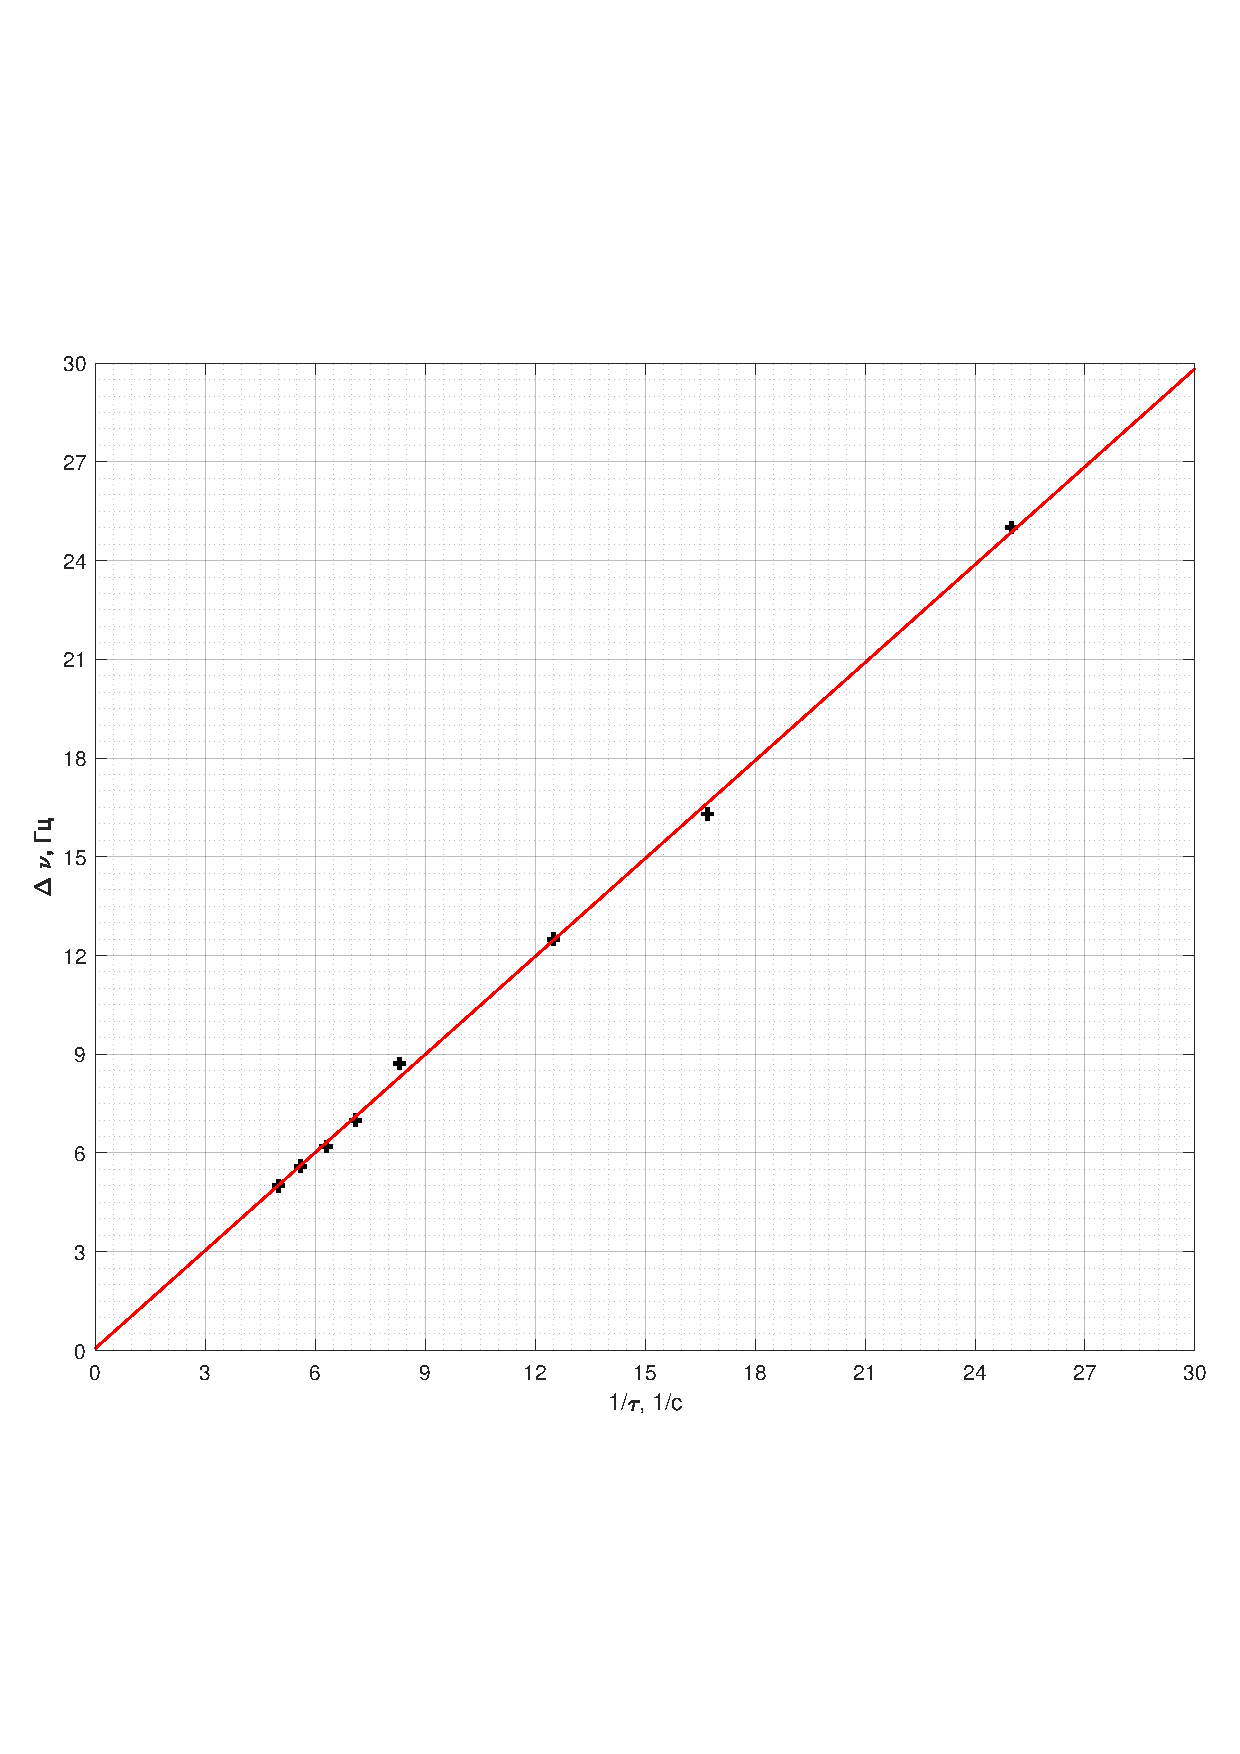
\includegraphics[width=\linewidth]{gr1.pdf}
	\caption{график зависимости $B(I)$}
	\label{gr1}
\end{figure}
\end{center}



По МНК находим, что: \[k_1 = (223 \pm 44)\dfrac{\text{мкН}}{\text{Тл}^2}, \ \ k_2 = (575 \pm 130)\dfrac{\text{мкН}}{\text{Тл}^2}\]


По формуле \eqref{eq1} рассчитаем что-то, погрешность рассчитываем по формуле:

Итого имеем
\[\text{что-то}_{\text{м}} = (-7.1 \pm 1.4) \cdot 10^{-6}, \ \  \text{что-то}_{\text{а}} = (18.4 \pm 4.2) \cdot 10^{-6}\]


(табличные значения для этих материалов: $\text{что-то}_{\text{м}} = -10.3 \cdot 10^{-6}, \ \  \text{что-то}_{\text{а}} = 23 \cdot 10^{-6}$)

\section*{Выводы}
\begin{enumerate}
	\item В ходе выполнения работы были расчитаны значения чего-то для меди и алюминия: $\text{что-то}_{\text{м}} = (-7.1 \pm 1.4) \cdot 10^{-6}, \  \text{что-то}_{\text{а}} = (18.4 \pm 4.2) \cdot 10^{-6}$, которые совпали с табличными значениями в пределах погрешности.
	\item Большая погрешность (20\% для меди и 23\% для алюминия) получилась вследствие больших неточностей в измерениях.
	\item Так как $\text{что-то}_{\text{м}} < 0$, а $\text{что-то}_{\text{а}} > 0$, можно сделать вывод, что медь -- это диамагнетик, а алюминий -- это парамагнетик.
\end{enumerate}


\end{document}